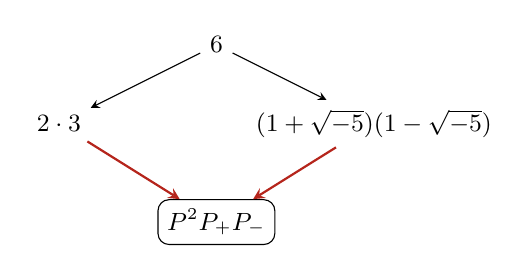
\begin{tikzpicture}[>=stealth,font=\small]
\node (six) at (0,0) {$6$};
\node (a) at (-2,-1) {$2\cdot3$};
\node (b) at (2,-1) {$(1+\sqrt{-5})(1-\sqrt{-5})$};
\node[draw,rounded corners] (c) at (0,-2.25) {$P^2P_+P_-$};
\draw[->] (six)--(a);\draw[->] (six)--(b);
\draw[->,BrickRed,thick] (a)--(c);\draw[->,BrickRed,thick] (b)--(c);
\end{tikzpicture}
